
\subsection{Deriving a power series for the NTK}\label{appendix:subsec:deriving_power_series}

We will require the following minor adaptation of \citet[Lemma D.2]{marco}. We remark this result was first stated for ReLU and Softplus activations in the work of \citet[Lemma H.2]{solt_mod_over}. 


\begin{lemma}\label{lemma:matrix_hermite_expansion}
    For arbitrary $n,d \in \naturals$, let $\mA \in \reals^{n \times d}$. For $i \in [n]$, we denote the $i$th row of $\mA$ as $\va_i$, and further assume that $\norm{\va_i} =1$. Let $\phi: \reals \rightarrow \reals$ satisfy $\phi \in L^2(\reals, \gamma)$ and define
    \[
    \mM = \expec_{\vw \sim \cN(0, \textbf{I}_{n})}[\phi(\mA\vw)\phi(\mA \vw)^T] \in \reals^{n \times n}.
    \]
    Then the matrix series
    \[
    \mS_K = \sum_{k = 0}^{K} \mu_k^2(\phi) \left(\mA \mA^T \right)^{\odot k}
    \]
    converges uniformly to $\mM$ as $K \rightarrow \infty$.
\end{lemma}
The proof of Lemma \ref{lemma:matrix_hermite_expansion} follows exactly as in \cite[Lemma D.2]{marco}, and is in fact slightly simpler due to the fact we assume the rows of $\mA$ are unit length and $\vw \sim \cN(0, \textbf{I}_d)$ instead of $\sqrt{d}$ and $\vw \sim \cN(0, \frac{1}{d}\textbf{I}_d)$ respectively. For the ease of the reader, we now recall the following definitions, which are also stated in Section \ref{sec:power_series}. Letting $\bar{\alpha}_l \defeq (\alpha_{p,l})_{p=0}^{\infty}$ denote a sequence of real coefficients, then
    \begin{equation}
            F(p,k,\bar{\alpha}_{l}) \defeq 
            \begin{cases}
                1 \; &k=0 \text{ and } p = 0, \\
                0 \; &k=0 \text{ and } p \geq 1,\\
                \sum_{(j_i) \in \cJ(p,k)} \prod_{i=1}^k \alpha_{j_i, l} \; &k\geq 1 \text{ and } p \geq 0,
            \end{cases}
    \end{equation}
    where
    \[
    \cJ(p,k) \defeq \{ (j_i)_{i \in [k]} \; : \; j_i \geq 0 \; \forall i \in [k], \; \sum_{i=1}^k j_i = p  \} 
    \]
    for all $p \in \ints_{\geq 0}$, $k \in \ints_{\geq 1}$. 
    
We are now ready to derive power series for elements of $(\mG_l))_{l=1}^{L+1}$ and $(\dot{\mG}_l))_{l=2}^{L+1}$. 

\begin{lemma} \label{lemma:power_series_G}
     Under Assumptions \ref{assumptions:kernel_regime} and \ref{assumption:init_var_1}, for all $l \in [2,L+1]$
    \begin{equation}\label{eq:recurrence_G}
        \begin{aligned}
            &\mG_{l} = \sum_{k=0}^{\infty} \alpha_{k,l}(\mX\mX^T)^{\odot k},
        \end{aligned}
    \end{equation}
    where the series for each element $[\mG_{l}]_{ij}$ converges absolutely and the coefficients $\alpha_{p,l}$ are nonnegative.
    The coefficients of the series \eqref{eq:recurrence_G} for all $p\in \ints_{\geq 0}$ can be expressed via the following recurrence relationship, 
    \begin{equation}\label{eq:recurrence_G_coeffs}
        \alpha_{p,l} = 
        \begin{cases}
            \sigma_w^2 \mu_p^2(\phi) + \delta_{p=0}\sigma_b^2, &l=2,\\
            \sum_{k=0}^{\infty}\alpha_{k,2} F(p,k,\bar{\alpha}_{l-1}), &l\geq 3.
        \end{cases}
    \end{equation}
    Furthermore,
    \begin{equation} \label{eq:recurrence_Gdot}
        \begin{aligned}
            &\dot{\mG}_{l} = \sum_{k=0}^{\infty} \upsilon_{k,l}(\mX\mX^T)^{\odot k},
        \end{aligned}
    \end{equation}
    where likewise the series for each entry $[\dot{\mG}_{l}]_{ij}$ converges absolutely and the coefficients $\upsilon_{p,l}$ for all $p\in \ints_{\geq 0}$ are nonnegative and can be expressed via the following recurrence relationship, 
     \begin{equation}\label{eq:recurrence_Gdot_coeffs}
        \upsilon_{p,l} = 
        \begin{cases}
            \sigma_w^2 \mu_p^2(\phi'), &l=2,\\
            \sum_{k=0}^{\infty} \upsilon_{k,2} F(p,k,\bar{\alpha}_{l-1}), &l\geq3.
        \end{cases}
    \end{equation}
\end{lemma}

\begin{proof}
    We start by proving \eqref{eq:recurrence_G} and \eqref{eq:recurrence_G_coeffs}. Proceeding by induction, consider the base case $l=2$. From Lemma \ref{lemma:ntk_exp1}
    \[
        \mG_{2} = \sigma_w^2 \expec_{\vw \sim \cN(\textbf{0}, \textbf{I}_d)}[\phi(\mX \vw) \phi(\mX \vw)^T] + \sigma_b^2 \textbf{1}_{n \times n}.
    \]
    By the assumptions of the lemma, the conditions of Lemma \ref{lemma:matrix_hermite_expansion} are satisfied and therefore
    \[
    \begin{aligned}
        \mG_{2} &= \sigma_w^2 \sum_{k = 0}^{\infty} \mu_k^2(\phi) \left(\mX \mX^T \right)^{\odot k} + \sigma_b^2 \textbf{1}_{n\times n}\\
        & = \alpha_{0,2}\textbf{1}_{n \times n} + \sum_{k=1}^{\infty}\alpha_{k,2}\left(\mX \mX^T \right)^{\odot k}.
    \end{aligned}
    \]
    Observe the coefficients $(\alpha_{k,2})_{k \in \ints_{\geq 0}}$ are nonnegative. Therefore, for any $i,j \in [n]$ using Lemma~\ref{lemma:unit_var} the series for $[\mG_{l}]_{ij}$ satisfies 
    \begin{equation}\label{eq:absolute_convergence_G_entries}
    \begin{aligned}
        \sum_{k=0}^{\infty} \abs{\alpha_{k,2}} \abs{\langle \vx_i, \vx_j \rangle^{k}} 
        & \leq \sum_{k=0}^{\infty} \alpha_{k,2} \langle \vx_i, \vx_i \rangle^{k}
        & = [\mG_{l}]_{ii}
        & = 1
    \end{aligned}
    \end{equation}
    and so must be absolutely convergent. With the base case proved we proceed to assume the inductive hypothesis holds for arbitrary $\mG_{l}$ with $l \in [2,L]$. Observe
    \[
    \begin{aligned}
        \mG_{l+1}  &= \sigma_w^2 \expec_{\vw \sim \cN(\textbf{0}, \textbf{I}_n)}[\phi(\mA \vw) \phi(\mA \vw)^T] + \sigma_b^2 \textbf{1}_{n \times n},
    \end{aligned}
    \]
    where $\mA$ is a matrix square root of $\mG_{l}$, meaning $\mG_{l} = \mA \mA$. Recall from Lemma \ref{lemma:ntk_exp1} that $\mG_{l}$ is also symmetric and positive semi-definite, therefore we may additionally assume, without loss of generality, that $\mA \in \reals^{n \times n}$ is symmetric, which conveniently implies $\mG_{n,l} = \mA \mA^T$. Under the assumptions of the lemma the conditions for Lemma \ref{lemma:unit_var} are satisfied and as a result $[\mG_{n,l}]_{ii} = \norm{\va_i} = 1$ for all $i \in [n]$, where we recall $\va_i$ denotes the $i$th row of $\mA$. Therefore we may again apply Lemma \ref{lemma:ntk_exp1},
    \[
    \begin{aligned}
        \mG_{l+1}  &= \sigma_w^2 \sum_{k = 0}^{\infty} \mu_k^2(\phi) \left(\mA \mA^T \right)^{\odot k} + \sigma_b^2 \textbf{1}_{n\times n}\\
        &= (\sigma_w^2\mu_0^2(\phi) + \sigma_b^2) \textbf{1}_{n \times n} + \sigma_w^2\sum_{k=1}^{\infty}\mu_k^2(\phi)\left(\mG_{n,l}\right)^{\odot k}\\
        & = (\sigma_w^2\mu_0^2(\phi) + \sigma_b^2) \textbf{1}_{n \times n} + \sigma_w^2\sum_{k=1}^{\infty}\mu_k^2(\phi)\left(\sum_{m=0}^{\infty} \alpha_{m,l}(\mX\mX^T)^{\odot m}\right)^{\odot k},
    \end{aligned}
    \]
    where the final equality follows from the inductive hypothesis. For any pair of indices $i,j \in [n]$
    \[
    [\mG_{l+1}]_{ij} = (\sigma_w^2\mu_0^2(\phi) + \sigma_b^2) + \sigma_w^2\sum_{k=1}^{\infty}\mu_k^2(\phi)\left(\sum_{m=0}^{\infty} \alpha_{m,l}\langle \vx_i, \vx_j \rangle^m\right)^k.
    \]
     By the induction hypothesis, for any $i,j \in [n]$ the series $\sum_{m=0}^\infty\alpha_{m,l}\langle \vx_i, \vx_j \rangle^m$ is absolutely convergent. Therefore, from the Cauchy product of power series and for any $k \in \ints_{\geq 0}$ we have
     \begin{equation} \label{eq:cauchy_product}
     \left(\sum_{m=0}^{\infty} \alpha_{m,l}\langle \vx_i, \vx_j \rangle^m\right)^k = \sum_{p=0}^{\infty} F(p,k,\bar{\alpha}_{l}) \langle \vx_i, \vx_j \rangle^p,
     \end{equation}
    where $F(p,k,\bar{\alpha}_{l})$ is defined in \eqref{eq:def_F}. By definition, $F(p,k,\bar{\alpha}_{l})$ is a sum of products of positive coefficients, and therefore $\abs{F(p,k,\bar{\alpha}_{l})} = F(p,k,\bar{\alpha}_{l})$. In addition, recall again by Assumption \ref{assumption:init_var_1} and Lemma \ref{lemma:unit_var} that $[\mG_{l}]_{ii} = 1$. As a result, for any $k \in \ints_{\geq 0}$, as $\abs{\langle \vx_i, \vx_j \rangle} \leq 1$
    \begin{equation}\label{eq:capitalfsumsoverp}
    \sum_{p=0}^{\infty} \abs{F(p,k,\bar{\alpha}_{l}) \langle \vx_i, \vx_j \rangle^p} \leq \left(\sum_{m=0}^{\infty} \alpha_{m,l} \right)^k = [\mG_{n,l}]_{ii} = 1
    \end{equation}
     and therefore the series $\sum_{p=0}^{\infty} F(p,k,\bar{\alpha}_{l})\langle \vx_i, \vx_j \rangle^p $ converges absolutely. Recalling from the proof of the base case that the series $\sum_{p=1}^{\infty} \alpha_{p,2}$ is absolutely convergent and has only nonnegative elements, we may therefore interchange the order of summation in the following,
    \[
    \begin{aligned}
    [\mG_{l+1}]_{ij} &= (\sigma_w^2\mu_0^2(\phi) + \sigma_b^2) + \sigma_w^2\sum_{k=1}^{\infty}\mu_k^2(\phi)\left(\sum_{p=0}^{\infty} F(p,k,\bar{\alpha}_{l}) \langle \vx_i, \vx_j \rangle^p\right)\\
    & = \alpha_{0,2} + \sum_{k=1}^{\infty}\alpha_{k,2}\left(\sum_{p=0}^{\infty} F(p,k,\bar{\alpha}_{l}) \langle \vx_i, \vx_j \rangle^p\right)\\
    & = \alpha_{0,2} + \sum_{p=0}^{\infty} \left(\sum_{k=1}^{\infty}\alpha_{k,2} F(p,k,\bar{\alpha}_{l}) \right) \langle \vx_i, \vx_j \rangle^p . 
    \end{aligned}
    \]
    Recalling the definition of $F(p,k,l)$ in \eqref{eq:def_F}, in particular $F(0,0,\bar{\alpha}_l) = 1$ and $F(p,0,\bar{\alpha}_l) = 0$ for $p \in \ints_{\geq 1}$, then
    \[
    \begin{aligned}
     [\mG_{l+1}]_{ij} & = \left(\alpha_{0,2} + \sum_{k=1}^{\infty}\alpha_{k,2} F(0,k,\bar{\alpha}_l)\right) \langle \vx_i, \vx_j \rangle^0 + \sum_{p=1}^{\infty} \left(\sum_{k=1}^{\infty}\alpha_{k,2} F(p,k,\bar{\alpha}_{l}) \right) \langle \vx_i, \vx_j \rangle^p\\
    & = \left(\sum_{k=0}^{\infty}\alpha_{k,2} F(0, k, \bar{\alpha}_l)\right)\langle \vx_i, \vx_j \rangle^0 + \sum_{p=1}^{\infty} \left(\sum_{k=0}^{\infty}\alpha_{k,2} F(p,k,\bar{\alpha}_{l}) \right) \langle \vx_i, \vx_j \rangle^p\\
    & = \sum_{p=0}^{\infty} \left(\sum_{k=0}^{\infty}\alpha_{k,2} F(p,k,\bar{\alpha}_{l}) \right) \langle \vx_i, \vx_j \rangle^p\\
    & = \sum_{p=0}^{\infty} \alpha_{p, l+1} \langle \vx_i, \vx_j \rangle^p.
    \end{aligned}
    \]
    As the indices $i,j \in [n]$ were arbitrary we conclude that
    \[
    \mG_{l+1} = \sum_{p=0}^{\infty} \alpha_{p, l+1} \left( \mX \mX^T\right)^{\odot p}
    \]
    as claimed. In addition, by inspection and using the induction hypothesis it is clear that the coefficients $(\alpha_{p,l+1})_{p=0}^{\infty}$ are nonnegative. Therefore, by an argument identical to \eqref{eq:absolute_convergence_G_entries}, the series for each entry of $[\mG_{l+1}]_{ij}$ is absolutely convergent. This concludes the proof of \eqref{eq:recurrence_G} and \eqref{eq:recurrence_G_coeffs}. 
    
    We now turn our attention to proving the \eqref{eq:recurrence_Gdot} and \eqref{eq:recurrence_Gdot_coeffs}.  Under the assumptions of the lemma the conditions for Lemmas \ref{lemma:ntk_exp1} and \ref{lemma:matrix_hermite_expansion} are satisfied and therefore for the base case $l=2$ 
    \[
    \begin{aligned}
        \dot{\mG}_{2} &= \sigma_w^2 \expec_{\vw \sim \cN(\textbf{0}, \textbf{I}_n)}[\phi'(\mX \vw) \phi'(\mX \vw)^T]\\
        &= \sigma_w^2 \sum_{k=0}^\infty \mu_k^2(\phi') \left(\mX \mX^T \right)^{\odot k}\\
        & = \sum_{k=0}^\infty \upsilon_{k,2} \left(\mX \mX^T \right)^{\odot k}. 
    \end{aligned}
    \]
    By inspection the coefficients $(\upsilon_{p,2})_{p=0}^{\infty}$ are nonnegative and as a result by an argument again identical to \eqref{eq:absolute_convergence_G_entries} the series for each entry of $[\dot{\mG}_{2}]_{ij}$ is absolutely convergent. For $l \in [2,L]$, from \eqref{eq:recurrence_G} and its proof there is a matrix $\mA \in \reals^{n \times n}$ such that $\mG_{l} = \mA \mA^T$. Again applying Lemma \ref{lemma:matrix_hermite_expansion}
    \[
    \begin{aligned}
    \dot{\mG}_{n,l+1}
    & = \sigma_w^2 \expec_{\vw \sim \cN(\textbf{0}, \textbf{I}_n)}[\phi'(\mA \vw) \phi'(\mA \vw)^T]\\
    & = \sigma_w^2 \sum_{k=0}^\infty \mu_k^2(\phi') \left(\mA \mA^T \right)^{\odot k}\\
    & = \sum_{k=0}^\infty \upsilon_{k,2}\left(\mG_{n,l}\right)^{\odot k}\\
    & = \sum_{k=0}^\infty \upsilon_{k,2}\left(\sum_{p=0}^{\infty} \alpha_{p, l} \left( \mX \mX^T\right)^{\odot p}\right)^{\odot k}
    \end{aligned}
    \]
    Analyzing now an arbitrary entry $[\dot{\mG}_{l+1}]_{ij}$, by substituting in the power series expression for $\mG_{l}$ from \eqref{eq:recurrence_G} and using \eqref{eq:cauchy_product} we have
    \[
    \begin{aligned}
        [\dot{\mG}_{l+1}]_{ij} &= \sum_{k=0}^\infty \upsilon_{k,2} \left(\sum_{p=0}^{\infty} \alpha_{p, l}  \langle \vx_i, \vx_j \rangle^p \right)^k\\
        & = \sum_{k=0}^\infty \upsilon_{k,2} \left(\sum_{p=0}^{\infty} F(p,k,\bar{\alpha}_{l}) \langle \vx_i, \vx_j \rangle^p \right)\\
        & = \sum_{p=0}^{\infty} \left(\sum_{k=0}^\infty\upsilon_{k,2} F(p,k,\bar{\alpha}_{l})\right)\langle \vx_i, \vx_j \rangle^p\\
        & = \sum_{p=0}^{\infty} \upsilon_{p, l+1}\langle \vx_i, \vx_j \rangle^p.
    \end{aligned}
    \]
    Note that exchanging the order of summation in the third equality above is justified as for any $k \in \ints_{\geq 0}$ by \eqref{eq:capitalfsumsoverp} we have $\sum_{p=0}^{\infty} F(p,k,\bar{\alpha}_{l}) |\langle \vx_i, \vx_j \rangle|^p \leq 1$ and therefore $\sum_{k=0}^\infty \sum_{p=0}^{\infty}\upsilon_{k,2} F(p,k,\bar{\alpha}_{l}) \langle \vx_i, \vx_j \rangle^p$ converges absolutely. As the indices $i,j \in [n]$ were arbitrary we conclude that
    \[
        \dot{\mG}_{l+1} = \sum_{p=0}^{\infty} \upsilon_{p, l+1} \left(\mX \mX^T \right)^{\odot p}
    \]
    as claimed. Finally, by inspection the coefficients $(\upsilon_{p,l+1})_{p=0}^{\infty}$ are nonnegative, therefore, and again by an argument identical to \eqref{eq:absolute_convergence_G_entries}, the series for each entry of $[\dot{\mG}_{n,l+1}]_{ij}$ is absolutely convergent. This concludes the proof.
\end{proof}


We are now prove the key result of Section \ref{sec:power_series}.

\ntkPowerSeries* 

\begin{proof}
   We proceed by induction. The base case $l=1$ follows trivially from Lemma \ref{lemma:ntk_exp1}. We therefore assume the induction hypothesis holds for an arbitrary $l-1 \in [1,L]$. From \eqref{eq:reccurence_NTK_matrices} and Lemma \ref{lemma:power_series_G}
   \[
   \begin{aligned}
   n\mK_{l} &= \mG_{l} + n\mK_{l-1}\odot \dot{\mG}_{l}\\
   &= \left(\sum_{p = 0}^{\infty} \alpha_{p,l}\left( \mX \mX^T\right)^{\odot p}\right) + \left(n \sum_{q=0}^{\infty} \kappa_{q,l-1}\left( \mX \mX^T \right)^{\odot q}\right)\odot \left(\sum_{w=0}^{\infty} \upsilon_{w,l}\left( \mX \mX^T \right)^{\odot w}\right).
   \end{aligned}
   \]
   Therefore, for arbitrary $i,j \in [n]$
   \[
   \begin{aligned}
   [n\mK_{l}]_{ij}
   &= \sum_{p = 0}^{\infty} \alpha_{p,l}\langle\vx_i, \vx_j \rangle^p + \left( n\sum_{q=0}^{\infty} \kappa_{q,l-1}\langle\vx_i, \vx_j \rangle^q\right) \left(\sum_{w=0}^{\infty} \upsilon_{w,l}\langle\vx_i, \vx_j \rangle^w\right).
   \end{aligned}
   \]
   Observe $n\sum_{q=0}^{\infty} \kappa_{q,l-1}\langle\vx_i, \vx_j \rangle^q = \Theta^{(l-1)}(\vx_i, \vx_j)$ and therefore the series must converge due to the convergence of the NTK. Furthermore, $\sum_{w=0}^{\infty} \upsilon_{w,l}\langle\vx_i, \vx_j \rangle^w = [\dot{\mG}_{n,l}]_{ij}$ and therefore is absolutely convergent by Lemma \ref{lemma:power_series_G}. As a result, by Merten's Theorem the product of these two series is equal to their Cauchy product. Therefore
   \[
   \begin{aligned}
   [n\mK_{l}]_{ij}
   &= \sum_{p = 0}^{\infty} \alpha_{p,l}\langle\vx_i, \vx_j \rangle^p + \sum_{p=0}^{\infty} \left(\sum_{q = 0}^p \kappa_{q,l-1}\upsilon_{p-q,l} \right)\langle\vx_i, \vx_j \rangle^p\\
   &=\sum_{p = 0}^{\infty} \left( \alpha_{p,l} + \sum_{q = 0}^p \kappa_{q,l-1}\upsilon_{p-q,l}\right) \langle\vx_i, \vx_j \rangle^p\\
   & = \sum_{p = 0}^{\infty} \kappa_{p,l}\langle\vx_i, \vx_j \rangle^p,
   \end{aligned}
   \]
   from which the \eqref{eq:ntk_power_series} immediately follows.
\end{proof}


\subsection{Analyzing the coefficients of the NTK power series} \label{appendix:subsec:analyzing_ntk_coefficients}
In this section we study the coefficients of the NTK power series stated in Theorem \ref{theorem:ntk_power_series}. Our first observation is that, under additional assumptions on the activation function $\phi$, the recurrence relationship \eqref{eq:recurrence_ntk_coeffs} can be simplified in order to depend only on the Hermite expansion of $\phi$.

\begin{lemma}\label{lem:derivhermiterelation}
Under Assumption \ref{assumption:phi} the Hermite coefficients of $\phi'$ satisfy
\[ \mu_k(\phi') = \sqrt{k + 1} \mu_{k + 1}(\phi) \]
for all $k \in \ints_{\geq 0}$.
\end{lemma}
\begin{proof}
Note for each $n \in \mathbb{N}$ as $\phi$ is absolutely continuous on $[-n, n]$ it is differentiable a.e. on $[-n, n]$.  It follows by the countable additivity of the Lebesgue measure that $\phi$ is differentiable a.e. on $\mathbb{R}$.  Furthermore, as $\phi$ is polynomially bounded we have $\phi \in L^2(\mathbb{R}, e^{-x^2 / 2} / \sqrt{2 \pi})$.  Fix $a > 0$. Since $\phi$ is absolutely continuous on $[-a, a]$ it is of bounded variation on $[-a, a]$.  Also note that $h_k(x) e^{-x^2 / 2}$ is of bounded variation on $[-a, a]$ due to having a bounded derivative.  Thus we have by Lebesgue-Stieltjes integration-by-parts (see e.g. \citealt[Chapter 3]{folland1999}) 
\begin{gather*}
\int_{-a}^a \phi'(x) h_k(x) e^{-x^2 / 2} dx \\
= \phi(a) h_k(a) e^{-a^2 / 2} - \phi(-a) h_k(-a) e^{-a^2 / 2} + \int_{-a}^a \phi(x) [x h_k(x) - h_k'(x)]e^{-x^2/2} dx \\
= \phi(a) h_k(a) e^{-a^2 / 2} - \phi(-a) h_k(-a) e^{-a^2 / 2} + \int_{-a}^a \phi(x) \sqrt{k + 1} h_{k + 1}(x) e^{-x^2 / 2} dx , 
\end{gather*}
where in the last line above we have used the fact that \eqref{eq:HP1} and \eqref{eq:HP2} imply that $x h_k(x) - h_k'(x) = \sqrt{k + 1} h_{k + 1}(x)$. 
Thus we have shown 
\begin{gather*}
\int_{-a}^a \phi'(x) h_k(x) e^{-x^2 / 2} dx \\
= \phi(a) h_k(a) e^{-a^2 / 2} - \phi(-a) h_k(-a) e^{-a^2 / 2} + \int_{-a}^a \phi(x) \sqrt{k + 1} h_{k + 1}(x) e^{-x^2 / 2} dx.   
\end{gather*}
We note that since $|\phi(x) h_k(x)| = \mathcal{O}(|x|^{\beta + k})$ we have that as $a \rightarrow \infty$ the first two terms above vanish.  Thus by sending $a \rightarrow \infty$ we have
\[ 
\int_{-\infty}^\infty \phi'(x) h_k(x) e^{-x^2 / 2} dx = \int_{-\infty}^\infty \sqrt{k + 1} \phi(x) h_{k + 1}(x) e^{-x^2 / 2} dx.
\]
After dividing by $\sqrt{2 \pi}$ we get the desired result. 
\end{proof}

In particular, under Assumption~\ref{assumption:phi}, and as highlighted by Corollary~\ref{corollary:upsilons_as_alphas}, which follows directly from Lemmas \ref{lemma:power_series_G} and \ref{lem:derivhermiterelation}, the NTK coefficients can be computed only using the Hermite coefficients of~$\phi$. 

\begin{corollary} \label{corollary:upsilons_as_alphas}
Under Assumptions \ref{assumptions:kernel_regime}, \ref{assumption:init_var_1} and \ref{assumption:phi}, for all $p \in \ints_{\geq 0}$
\begin{equation}\label{eq:recurrence_Gdot_coeffs_simple}
        \upsilon_{p,l} = 
        \begin{cases}
            (p+1)\alpha_{p+1,2}, &l=2,\\
            \sum_{k=0}^{\infty} \upsilon_{k,2} F(p,k,\bar{\alpha}_{l-1}), &l\geq 3.
        \end{cases}
\end{equation}
\end{corollary}

With these results in place we proceed to analyze the decay of the coefficients of the NTK for depth two networks. As stated in the main text, the decay of the NTK coefficients depends on the decay of the Hermite coefficients of the activation function deployed. This in turn is strongly influenced by the behavior of the tails of the activation function. To this end we roughly group activation functions into three categories: growing tails, flat or constant tails and finally decaying tails. Analyzing each of these groups in full generality is beyond the scope of this paper, we therefore instead study the behavior of ReLU, Tanh and Gaussian activation functions, being prototypical and practically used examples of each of these three groups respectively. We remark that these three activation functions satisfy Assumption \ref{assumption:phi}. For typographical ease we let $\omega_{\sigma}(z) \defeq (1/\sqrt{2 \pi \sigma^2}) \exp\left( -z^2/ (2 \sigma^2)\right)$ denote the Gaussian activation function with variance $\sigma^2$.

\NTKcoeffTwolayer*

\begin{proof}
      Recall \eqref{eq:ntk_coeffs_2_layer_simple},
    \[
        \kappa_{p,2} = \sigma_w^2(1 + \gamma_w^2 p)\mu_p^2(\phi) +\sigma_w^2 \gamma_b^2(1+p) \mu_{p+1}^2(\phi)+ \delta_{p=0} \sigma_b^2.
    \]
    In order to bound $\kappa_{p,2}$ we proceed by using Lemma \ref{lemma:hermite_relu} to bound the square of the Hermite coefficients. We start with ReLU. Note Lemma \ref{lemma:hermite_relu} actually provides precise expressions for the Hermite coefficients of ReLU, however, these are not immediately easy to interpret. Observe from Lemma~\ref{lemma:hermite_relu} that above index $p=2$ all odd indexed Hermite coefficients are $0$. It therefore suffices to bound the even indexed terms, given by 
    \[
    \mu_p(ReLU) = \frac{1}{\sqrt{2 \pi}}\frac{(p-3)!!}{\sqrt{p!}}.
    \]
    Observe from \eqref{eq:HP3} that for $p$ even
    \[
    h_p(0) = (-1)^{p/2} \frac{(p-1)!!}{\sqrt{p!}}, 
    \]
    therefore
    \[
    \mu_p(ReLU) = \frac{1}{\sqrt{2 \pi}}\frac{(p-3)!!}{\sqrt{p!}} =  \frac{1}{\sqrt{2 \pi}} \frac{\abs{h_p(0)}}{p-1}.
    \]
    Analyzing now $\abs{h_p(0)}$, 
    \[ \frac{(p - 1)!!}{\sqrt{p!}} = \frac{\prod_{i = 1}^{p/2} (2i - 1)}{\sqrt{\prod_{i = 1}^{p/2} (2i - 1) 2i}} = \sqrt{\frac{\prod_{i = 1}^{p/2} (2i - 1)}{\prod_{i = 1}^{p/2} 2i}} = \sqrt{\frac{(p - 1)!!}{p!!}}.\]
    Here, the expression inside the square root is referred to in the literature as the Wallis ratio, for which the following lower and upper bounds are available \cite{kazarinoff_1956},
    \begin{equation} \label{eq:wallis_ratio_bounds}
        \sqrt{\frac{1}{\pi(p+0.5)}} < \frac{(p - 1)!!}{p!!} < \sqrt{\frac{1}{\pi(p+0.25)}}.
    \end{equation}
    As a result
    \[
    \abs{h_p(0)} = \Theta(p^{-1/4})
    \]
    and therefore
    \[
    \mu_p(ReLU) = 
    \begin{cases}
        \Theta(p^{-5/4}), \; &p \text{ even},\\
        0, \; &p \text{ odd}.
    \end{cases}
    \]
    As $(p+1)^{-3/2} = \Theta(p^{-3/2})$, then from \eqref{eq:ntk_coeffs_2_layer_simple}  
    \[
    \begin{aligned}
        \kappa_{p,2}  &= \Theta(( p \mu_p^2(ReLU) + \delta_{\gamma_b>0}(p+1) \mu_{p+1}^2(ReLU)))\\
        & = \Theta(( \delta_{p \text{ even}}p^{-3/2} + \delta_{(p \text{ odd})\cap(\gamma_b>0)}(p+1)^{-3/2}))\\
        &= \Theta \left( \delta_{(p \text{ even}) \cup \left((p \text{ odd})\cap(\gamma_b>0)\right)}p^{-3/2}\right)\\
        & = \delta_{(p \text{ even}) \cup(\gamma_b>0)} \Theta \left( p^{-3/2}\right) 
    \end{aligned}
    \]
    as claimed in item \emph{1.} 
    
    We now proceed to analyze $\phi(z) = Tanh(z)$. From \citet[Corollary F.7.1]{Panigrahi2020Effect}
    \[
    \mu_p(Tanh') = \cO \left(\exp\left( - \frac{\pi \sqrt{p}}{4}\right)\right) . 
    \]
     As Tanh satisfies the conditions of Lemma~\ref{lem:derivhermiterelation}
    \[
    \mu_p(Tanh) = p^{-1/2} \mu_{p-1}(Tanh') = \cO \left( p^{-1/2}\exp\left( - \frac{\pi \sqrt{p-1}}{4}\right)\right).
    \]
    Therefore the result claimed in item \emph{2.} follows as
    \[
    \begin{aligned}
    \kappa_{p,2}  &= \cO((p\mu_p^2(Tanh) + (p+1)\mu_{p+1}^2(Tanh))) \\
    &= \cO \left( \exp\left( - \frac{\pi \sqrt{p-1}}{2}\right) + \exp\left( - \frac{\pi \sqrt{p}}{2}\right) \right)\\
    &= \cO \left( \exp\left( - \frac{\pi \sqrt{p-1}}{2}\right)\right).
    \end{aligned}
    \]
    Finally, we now consider $\phi(z) = \omega_{\sigma}(z)$ where $\omega_{\sigma}(z)$ is the density function of $\cN(0, \sigma^2)$. Similar to ReLU, analytic expressions for the Hermite coefficients of $\omega_{\sigma}(z)$ are known \citep[see e.g.,][Theorem 2.9]{davis_hermite}, 
    \[
    \mu_p^2(\omega_{\sigma}) = 
    \begin{cases}
        \frac{p!}{(\left(p/2\right)!)^2 2^{p}2 \pi (\sigma^2 + 1)^{p+1}}, \; &\text{p even},\\
        0, \; &\text{p odd}.\\
    \end{cases}
    \]
    For $p$ even
    \[
        (p/2)! = p!! 2^{-p/2}.
    \]
    Therefore
    \[
    \begin{aligned}
        \frac{p!}{(p/2)!(p/2)!} = 2^p\frac{p!}{p!! p!!}
        = 2^p \frac{(p-1)!!}{p!!}.
    \end{aligned}
    \]
    As a result, for $p$ even and using \eqref{eq:wallis_ratio_bounds}, it follows that
    \[
    \begin{aligned}
        \mu_p^2(\omega_{\sigma}) &= \frac{(\sigma^2+1)^{-(p+1)}}{2 \pi } \frac{(p-1)!!}{p!!}
        & = \Theta(p^{-1/2}(\sigma^2+1)^{-p}) . 
    \end{aligned}
    \] 
    Finally, since $(p+1)^{1/2}(\sigma^2+1)^{-p-1} = \Theta(p^{1/2}(\sigma^2+1)^{-p})$, then from \eqref{eq:ntk_coeffs_2_layer_simple}  
    \[
    \begin{aligned}
        \kappa_{p,2}  &= \Theta(( p \mu_p^2(\omega_{\sigma}) + \delta_{\gamma_b>0}(p+1) \mu_{p+1}^2(\omega_{\sigma})))\\
        &= \Theta \left( \delta_{(p \text{ even}) \cup \left((p \text{ odd})\cap(\gamma_b>0)\right)}p^{1/2}(\sigma^2+1)^{-p}\right)\\
        & = \delta_{(p \text{ even}) \cup(\gamma_b>0)} \Theta \left( p^{1/2}(\sigma^2+1)^{-p}\right)
    \end{aligned}
    \]
    as claimed in item \emph{3.} 
\end{proof}




\subsection{Numerical approximation via a truncated NTK power series and interpretation of Figure \ref{fig:error_truncated_ntk}} \label{appendix:numerical_approx_ntk}
Currently, computing the infinite width NTK requires either 
a) explicit evaluation of the Gaussian integrals highlighted in \eqref{eq:recurrence_G_matrices}, 
b) numerical approximation of these same integrals such as in \cite{LeeBNSPS18}, or 
c) approximation via a sufficiently wide yet still finite width network, see for instance \cite{torchNTK, pmlr-v162-novak22a}. These Gaussian integrals \eqref{eq:recurrence_G_matrices} can be solved solved analytically only for a minority of activation functions, notably ReLU as discussed for example by \cite{arora_exact_comp}, while the numerical integration and finite width approximation approaches are relatively computationally expensive.
The truncated NTK power series we define as analogous to \eqref{eq:ntk_power_series} but with the series involved being computed only up to the $T$th element. Once the top $T$ coefficients are computed, then for any input correlation the NTK can be approximated by evaluating the corresponding finite degree $T$ polynomial.

\begin{definition} \label{def:truncated_ntk}
    For an arbitrary pair $\vx, \vy \in \sphere^{d-1}$ let $\rho = \vx^T\vy$ denote their linear correlation. Under Assumptions \ref{assumptions:kernel_regime}, \ref{assumption:init_var_1} and \ref{assumption:phi}, for all $l \in [2, L+1]$ the $T$-truncated NTK power series $\hat{\Theta}_{T}^{(l)}:[-1,1]\rightarrow \reals$ is defined as
    \begin{equation}
        \Theta_T^{(l)}(\rho) = \sum_{p=0}^T \hat{\kappa}_{p,l} \rho^p.
    \end{equation}
    and whose coefficients are defined via the following recurrence relation,
    \begin{equation}
        \hat{\kappa}_{p,l} = 
        \begin{cases}
            \delta_{p=0}\gamma_b^2 + \delta_{p=1}\gamma_w^2, & l=1,\\
            \hat{\alpha}_{p,l} + \sum_{q = 0}^p \hat{\kappa}_{q,l-1}\hat{\upsilon}_{p-q,l}, &l \in [2,L+1].
        \end{cases}
    \end{equation}
    Here, with $\bar{\hat{\alpha}}_{l-1} = (\hat{\alpha}_{p,l-1})_{p=0}^T$,
    \begin{equation}
        \hat{\alpha}_{p,l} \defeq 
        \begin{cases}
            \sigma_w^2 \mu_p^2(\phi) + \delta_{p=0}\sigma_b^2, &l=2,\\
            \sum_{k=0}^{T} \hat{\alpha}_{k,2} F(p,k,\bar{\hat{\alpha}}_{l-1}), &l\geq 3
        \end{cases}
    \end{equation}
    and
    \begin{equation}
        \hat{\upsilon}_{p,l} \defeq 
        \begin{cases}
            \sqrt{p+1}\hat{\alpha}_{p+1,2}, &l=2,\\
            \sum_{k=0}^{T} \sqrt{k+1} \hat{\alpha}_{p+1,2} F(p,k,\bar{\hat{\alpha}}_{l}), &l\geq 3.
        \end{cases}
    \end{equation}
\end{definition}

In order to analyze the performance and potential of the truncated NTK for numerical approximation, we compute it for ReLU and compare it with its analytical expression \cite{arora_exact_comp}. To recall this result, let
\[
\begin{aligned}
    R(\rho) &\defeq \frac{\sqrt{1-\rho^2} + \rho \cdot \arcsin(\rho)}{\pi} + \frac{\rho}{2},\\
    R'(\rho) &\defeq \frac{\arcsin(\rho)}{\pi} + \frac{1}{2}.
\end{aligned}
\]
Under Assumptions \ref{assumptions:kernel_regime} and \ref{assumption:init_var_1}, with $\phi(z) = ReLU(z)$, $\gamma_w^2 = 1$, $\sigma_w^2 = 2$, $\sigma_b^2 = \gamma_b^2 = 0$, $\vx, \vy \in \sphere^d$ and $\rho_1 \defeq \vx^T\vy$, then $\Theta_1(\vx,\vy) = \rho$ and for all $l \in [2,L+1]$
\begin{equation}
    \begin{aligned}
        &\rho_l = R(\rho_{l-1}),\\
        &\Theta_l(\vx, \vy) = \rho_l + \rho_{l-1}R'(\rho_{l-1}).
    \end{aligned}
\end{equation}
Turning our attention to Figure \ref{fig:error_truncated_ntk}, we observe particularly for input correlations $\abs{\rho} \approx 0.5$ and below then the truncated ReLU NTK power series achieves machine level precision. For $\abs{\rho} \approx 1$ higher order coefficients play a more significant role. As the truncated ReLU NTK power series approximates these coefficients less well the overall approximation of the ReLU NTK is worse. We remark also that negative correlations have a smaller absolute error as odd indexed terms cancel with even index terms: we emphasize again that in Figure \ref{fig:error_truncated_ntk} we plot the absolute not relative error. In addition, for $L=1$ there is symmetry in the absolute error for positive and negative correlations as $\alpha_{p,2} = 0$ for all odd $p$. One also observes that approximation accuracy goes down with depth, which is due to the error in the coefficients at the previous layer contributing to the error in the coefficients at the next, thereby resulting in an accumulation of error with depth. Also, and certainly as one might expect, a larger truncation point $T$ results in overall better approximation. Finally, as the decay in the Hermite coefficients for ReLU is relatively slow, see e.g., Table~\ref{tab:kappa_2layer_coeffs} and Lemma~\ref{lemma:ntk_2layer_coeff_decay}, we expect the truncated ReLU NTK power series to perform worse relative to the truncated NTK's for other activation functions.

\begin{figure}[ht]
    \centering
    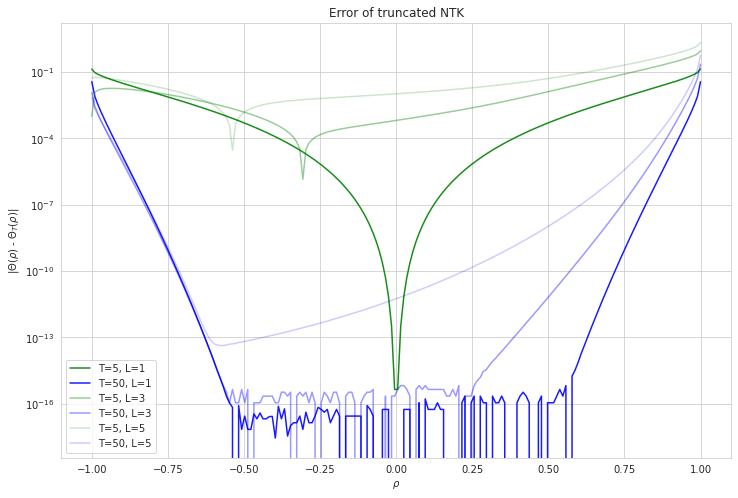
\includegraphics[width=0.8\textwidth]{conference_files/images/error_truncated_ntk.png}
    \caption{\textbf{(NTK Approximation via Truncation)} Absolute error between the analytical ReLU NTK and the truncated ReLU NTK power series as a function of the input correlation $\rho$ for two different values of the truncation point $T$ and three different values for the depth $L$ of the network. Although the truncated NTK achieves a uniform approximation error of only $10^{-1}$ on $[-1,1]$, for $\abs{\rho} \leq 0.5$, which we remark is more typical for real world data, $T=50$ suffices for the truncated NTK to achieve machine level precision.
    } 
    \label{fig:error_truncated_ntk}
\end{figure}


% \subsection{The zeroth coefficient of the NTK strictly increases with depth}\label{appendix:subsec:depth_effective_rank}
% The following lemmas show, somewhat unsurprisingly, that the zeroth coefficient of the NTK strictly grows with depth.

% \begin{lemma} \label{lemma:zeroth_coeff1}
%     Let the data, hyperparameters and activation function $\phi$ be such that Assumptions \ref{assumptions:kernel_regime}, \ref{assumption:init_var_1} and \ref{assumption:phi} are satisfied, and assume $\alpha_{0,2}>0$. Then for all $l\geq3$ it holds that $\alpha_{0,l}>\alpha_{0,l-1}$ and $\upsilon_{0,l}>\upsilon_{0,l-1}$.
% \end{lemma}

% \begin{proof}
%     We first consider the zeroth coefficients of the Gaussian Process kernel at each layer. From Theorem \ref{theorem:ntk_power_series} for $l\geq3$ recall that
%     \[
%         \alpha_{0,l} = \sum_{k=0}\alpha_{k,2}F(0,k, \bar{\alpha}_{l-1}) = \sum_{k=0}^{\infty} \alpha_{k,2}\alpha_{0,l-1}^k.
%     \]
%     We proceed by induction. For $l=3$ we have
%     \[
%     \alpha_{0,3} = \alpha_{0,2} + \sum_{k=1}^{\infty} \alpha_{k,2}\alpha_{0,2}^k.
%     \]
%     The base case $\alpha_{0,3}>\alpha_{0,2}$ is established by dividing both sides by $\alpha_{0,2}$ and recalling, again from Theorem \ref{theorem:ntk_power_series}, that the coefficients are nonnegative,
%     \[
%     \frac{\alpha_{0,3}}{\alpha_{0,2}} = 1 + \sum_{k=1}^{\infty} \alpha_{k,2}\alpha_{0,2}^{k-1} > 1.
%     \]
%     Assume now that the induction hypothesis holds at some layer $l\geq 3$, i.e., $\alpha_{0,l} > \alpha_{0, l-1}$. Then
%     \[
%     \alpha_{0,l+1} = \sum_{k=0}^{\infty} \alpha_{k,2}\alpha_{0,l}^k >\sum_{k=0}^{\infty} \alpha_{k,2}\alpha_{0,l-1}^k = \alpha_{0,l}
%     \]
%     and thus the inductive step is complete. We now turn our attention to analyzing the zeroth coefficient of the derivative of the Gaussian Process kernel. From Theorem \ref{theorem:ntk_power_series} and for $l\geq 3$
%     \[
%         \upsilon_{0,l} = \sum_{k=0}^{\infty}\upsilon_{k,2}F(0,k,\bar{\alpha}_{l-1}) = \sum_{k=0}^{\infty}\upsilon_{k,2} \alpha_{0,l-1}^k.
%     \]
%     The fact that $\upsilon_{0,3} > \upsilon_{0,2}$ follows as
%     \[
%      \frac{\upsilon_{0,3}}{\upsilon_{0,2}} = 1 + \sum_{k=1}^{\infty} \frac{\upsilon_{k,2}}{\upsilon_{0,2}}\alpha_{0,2}^k > 1
%     \]
%     For $l \geq 3$, as $\alpha_{0,l}>\alpha_{0,l-1}$, then the inequality $\upsilon_{0,l+1} > \upsilon_{0,l}$ can be derived by observing
%     \[
%     \upsilon_{0,l+1} = \sum_{k=0}^{\infty}\upsilon_{k,2} \alpha_{0,l}^k > \sum_{k=0}^{\infty}\upsilon_{k,2} \alpha_{0,l-1}^k = \upsilon_{0,l}.
%     \]
% \end{proof}

% \begin{lemma}\label{lemma:zeroth_coeff2}
%     Let the data, hyperparameters and activation function $\phi$ be such that Assumptions \ref{assumptions:kernel_regime}, \ref{assumption:init_var_1} and \ref{assumption:phi} are satisfied. Furthermore, assume the choice of hyperparameters and activation function are such that they satisfy the inequality $\sigma_w^2\mu_0^2(\phi) + \sigma_b^2 + \gamma_b^2 \sigma_w^2 \mu_1^2(\phi) > \gamma_b^2$. Then for all $l \geq 2$ it follows that $\kappa_{0,l}>\kappa_{0, l-1}$.
% \end{lemma}

% \begin{proof}
%     Observe, under the assumptions of the lemma, from Theorem \ref{theorem:ntk_power_series}  
%     \[
%         \kappa_{0,l} = \alpha_{0,l} + \kappa_{0,l-1}\upsilon_{0,l} = \alpha_{0,l} + \kappa_{0,l-1}\alpha_{1,l}.
%     \]
%     We proceed by induction. For the base case $l=2$ observe
%     \[
%         \kappa_{0,2} = \alpha_{0,2} + \kappa_{0,1}\alpha_{1,2} = \sigma_w^2\mu_0^2(\phi) + \sigma_b^2 + \gamma_b^2 \sigma_w^2 \mu_1^2(\phi) > \gamma_b^2 = \kappa_{0,1}.
%     \]
%     For the inductive step, assume that $\kappa_{0,l}>\kappa_{0,l-1}$ for some $l\geq 2$. Then using Lemma \ref{lemma:zeroth_coeff1}
%     \[
%     \kappa_{0,l+1} = \alpha_{0,l+1} + \kappa_{0,l}\upsilon_{0,l+1} > \alpha_{0,l} + \kappa_{0,l-1} \upsilon_{0,l} = \kappa_{0,l}. 
%     \]
%     This concludes the proof.
% \end{proof}

% Recalling the upper bound in Theorem \ref{thm:infinite_effective_constant_bd} and Corollary \ref{cor:trace_with_depth}, then, under additional assumptions on the activation function and by comparing the size of $\kappa_{0,l+1}$ relative to $\kappa_{0,l}(1 + \frac{1}{l})$,
% one could potentially characterize the impact of depth on the upper bound of the effective rank. We leave such analyses to future work.


\subsection{Characterizing NTK power series coefficient decay rates for deep networks} \label{subsec:appendix:deep_decay}
In general, Theorem \ref{theorem:ntk_power_series} does not provide a straightforward path to analyzing the decay of the NTK power series coefficients for depths greater than two. This is at least in part due to the difficulty of analyzing $F(p,k,\bar{\alpha}_{l-1})$, which recall is the sum of all ordered products of $k$ elements of $\bar{\alpha}_{l-1}$ whose indices sum to $p$, defined in \eqref{eq:def_F}. However, in the setting where the squares of the Hermite coefficients, and therefore the series $(\alpha_{p,2})_{p=0}^{\infty}$, decay at an exponential rate, this quantity can be characterized and therefore an analysis, at least to a certain degree, of the impact of depth conducted. Although admittedly limited in scope, we highlight that this setting is relevant for the study of Gaussian activation functions and radial basis function (RBF) networks.  We will also make the additional simplifying assumption that the activation function has zero Gaussian mean (which can be obtained by centering).  Unfortunately this further reduces the applicability of the following results to activation functions commonly used in practice. We leave the study of relaxing this zero bias assumption, perhaps only enforcing exponential decay asymptotically, as well as a proper exploration of other decay patterns, to future work.

The following lemma precisely describes, in the specific setting considered here, the evolution of the coefficients of the Gaussian Process kernel with depth. 

\begin{lemma} \label{lemma:deep_alpha_coeffs}
    Let $\alpha_{0,2} = 0$ and $\alpha_{p,2} = C_2 \eta_2^{-p}$ for $p \in \ints_{\geq 1}$, where $C_2$ and $\eta_2$ are constants such that $\sum_{p=1}^{\infty} \alpha_{p,2} = 1$. Then for all $l\geq 2$ and $p \in \ints_{\geq 0}$  \begin{equation}\label{eq:deep_exp_induction_hypothesis}
    \alpha_{p,l+1} = 
         \begin{cases}
            0, & \; p=0,\\
            C_{l+1} \eta_{l+1}^{-p}, & \;p \geq 1
        \end{cases}
    \end{equation}
    where the constants $\eta_{l+1}$ and $C_{l+1}$ are defined as
    \begin{equation}
    \begin{aligned} \label{eq:recurrence_C_eta}
        \eta_{l+1} = \frac{\eta_l \eta_2}{\eta_2 + C_l}, \;\; 
        C_{l+1} = \frac{C_l C_2}{\eta_2 + C_l}.
    \end{aligned}
    \end{equation}
\end{lemma}

\begin{proof}
Observe for $l=2$, we have that $\alpha_{0,l} = 0$ and $\alpha_{p, l} = C_l \eta_l^{-p}$ hold by assumption.  Thus by induction it suffices to show that $\alpha_{0, l} = 0$ and $\alpha_{p, l} = C_l \eta_l^{-p}$ implies \eqref{eq:deep_exp_induction_hypothesis} and \eqref{eq:recurrence_C_eta} hold.  Thus assume for some $l \geq 2$ we have that $\alpha_{0, l} = 0$ and $\alpha_{p, l} = C_l \eta_l^{-p}$. 
 Recall the definition of $F$ from \eqref{eq:def_F}: as $\alpha_{0,l} = 0$ then with $p \geq 1$ and $1 \leq k \leq p$
\[
F(p,k,\bar{\alpha}_l) = \sum_{(j_i) \in \cJ(p,k)} \prod_{i=1}^k \alpha_{j_i,l} = \sum_{(j_i) \in \cJ_{+}(p,k)} \prod_{i=1}^k \alpha_{j_i,l},
\]
where
\[
    \cJ_{+}(p,k) \defeq \big\{ (j_i)_{i \in [k]} \; : \; j_i \geq 1 \; \forall i \in [k], \; \sum_{i=1}^k j_i = p  \big\} \quad \text{for all $p \in \ints_{\geq 1}$, $k \in [p]$},
\]
which is the set of all $k$-tuples of \textit{positive} (instead of non-negative) integers which sum to $p$. Substituting $\alpha_{p,l} = C_l \eta_l^{-p}$ then
\[
    F(p,k,\bar{\alpha}_l) = \sum_{(j_i) \in \cJ_{+}(p,k)} C_l^k \eta_l^{-p} = C_l^k \eta_l^{-p} |\cJ_{+}(p,k)| =C_l^k \eta_l^{-p} \binom{p-1}{k-1}, 
\]
where the final equality follows from a stars and bars argument. Now observe for $k > p$ that at least one of the indices in $(j_i)_{i=1}^k$ must be 0 and therefore $\prod_{i=1}^k \alpha_{j_i,2} = 0$. As a result under the assumptions of the lemma
\begin{equation} \label{eq:F_at_layer3}
    F(p,k,\bar{\alpha}_l) = 
    \begin{cases}
        1, \; &k=0 \text{ and } p = 0, \\
        C_l^k \eta_l^{-p} \binom{p-1}{k-1}, \; & \; k \in [p] \text{ and } p \geq 1,\\
         0, \; &\text{ otherwise.}\\
    \end{cases}
\end{equation}
Substituting \eqref{eq:F_at_layer3} into \eqref{eq:recurrence_alpha_coeffs} it follows that
\[
\alpha_{0,l+1}  = \sum_{k=0}^{\infty} \alpha_{k,2} F(0,k,\bar{\alpha}_{l}) = \alpha_{0,2} = 0
\]
and for $p \geq 1$
\[
\begin{aligned}
\alpha_{p,l+1} &= \sum_{k=0}^{\infty} \alpha_{k,2} F(p,k,\bar{\alpha}_{l})\\
& = C_2 \eta_l^{-p} \sum_{k=1}^p  \left(\frac{C_l}{\eta_2} \right)^{k}  \binom{p-1}{k-1}\\
& = \eta_l^{-p} C_l \eta_2^{-1} C_2 \sum_{h=0}^{p-1} \left(\frac{C_l}{\eta_2} \right)^{h}\binom{p-1}{h}\\
& = \eta_l^{-p} C_l \eta_2^{-1} C_2 \left(1 + \frac{C_l}{\eta_2} \right)^{p-1}\\
& = \frac{C_l C_2}{\eta_2 + C_l} \left(\frac{\eta_l \eta_2}{\eta_2 + C_l}\right)^{-p}\\
& = C_{l+1} \eta_{l+1}^{-p}
\end{aligned}
\]
as claimed.
\end{proof}



We now analyze the coefficients of the derivative of the Gaussian Process kernel.

\begin{lemma} \label{lemma:deep_upsilon_coeffs}
    In addition to the assumptions of Lemma \ref{lemma:deep_alpha_coeffs}, assume also that $\phi$ satisfies Assumption \ref{assumption:phi}. Then $\upsilon_{p,2} = \frac{C_2}{\eta_2}(1+ p) \eta_2^{-p}$. Furthermore, for all $l\geq 2$ and $p \in \ints_{\geq 0}$  \begin{equation}\label{eq:deep_upsilon_hypothesis}
    \upsilon_{p,l+1} = 
         \begin{cases}
            C_2 \eta_2^{-1}, & \; p=0,\\
            (V_{l+1}' + V_{l+1}p)\eta_{l+1}^{-p}, & \;p \geq 1,
        \end{cases}
    \end{equation}
    where the constants $V_{l+1}'$ and $V_{l+1}$ are defined as
    \begin{equation}
    \begin{aligned} \label{eq:K_upsilon}
        V_{l+1}' \defeq \frac{2C_2 C_l}{\eta_2(C_l + \eta_2)} - \frac{C_2C_l^2}{\eta_2( C_l + \eta_2)^2}, \;\; V_{l+1} \defeq \frac{C_2C_l^2}{\eta_2( C_l + \eta_2)^2}    
    \end{aligned}
    \end{equation}
    and $C_l$ and $\eta_l$ are defined in \eqref{eq:recurrence_C_eta}.
\end{lemma}
\begin{proof}
    Under Assumption \ref{assumption:phi} then for all $p\in \ints_{\geq 0}$ we have
    \[
        \upsilon_{p,2} = \sigma_w^2 \mu_p^2(\phi') = \sigma_w^2 (p + 1) \mu_{p + 1}(\phi)^2 = (p+1)\alpha_{p+1,2} = \frac{C_2}{\eta_2}(1+ p) \eta_2^{-p}.
    \]
    For $l\geq 2$ and $p=0$ it therefore follows that
    \[
        \upsilon_{0,l+1} =  \sum_{k=0}^{\infty}(k+1)\alpha_{k+1,2} F(0,k,\bar{\alpha}_l)  = \alpha_{1,2} = C_2 \eta_2^{-1}.
    \]
    For $l\geq 2$ and $p\geq 1$ then
    \[
    \begin{aligned}
         \upsilon_{p,l+1} &= \sum_{k=0}^{\infty} \upsilon_{k,2} F(p,k,\bar{\alpha}_l)\\
         &= \sum_{k=0}^{\infty}(k+1)\alpha_{k+1,2} F(p,k,\bar{\alpha}_l)\\
        &= \sum_{h=1}^{\infty} h C_2 \eta_2^{-h} F(p,h-1,\bar{\alpha}_l)\\
        &=  \frac{C_2 }{C_l} \eta_l^{-p} \sum_{h=2}^{p+1} h \left(\frac{C_l}{\eta_2 }\right)^{ h}\binom{p-1}{h-2}\\
        & = \frac{C_2 }{C_l} \eta_l^{-p} \sum_{r=0}^{p-1} (r+2) \left(\frac{C_l}{\eta_2 }\right)^{ r+2}\binom{p-1}{r}\\
        & =  \frac{C_2 C_l}{\eta_2^2} \eta_l^{-p}\left(2 \sum_{r=0}^{p-1} \left(\frac{C_l}{\eta_2 }\right)^{ r}\binom{p-1}{r}   + \sum_{r=0}^{p-1} r \left(\frac{C_l}{\eta_2 }\right)^{ r}\binom{p-1}{r}\right)\\
        &=\frac{C_2 C_l}{\eta_2^2} \eta_l^{-p}\left(2 \left(1+ \frac{C_l}{\eta_2} \right)^{p-1} + \frac{C_l}{\eta_2}(p-1)\left(1 + \frac{C_l}{\eta_2} \right)^{p-2}\right)\\
        &= \frac{2C_2 C_l}{\eta_2(C_l + \eta_2)}\left(\frac{\eta_l \eta_2}{\eta_2 + C_l}\right)^{-p} + \frac{C_2C_l^2}{\eta_2( C_l + \eta_2)^2} (p-1) \left(\frac{\eta_l \eta_2}{\eta_2 + C_l}\right)^{-p}\\
        & = \left(\frac{2C_2 C_l}{\eta_2(C_l + \eta_2)} - \frac{C_2C_l^2}{\eta_2( C_l + \eta_2)^2} \right) \eta_{l+1}^{-p} + \left( \frac{C_2C_l^2}{\eta_2( C_l + \eta_2)^2}\right) p \eta_{l+1}^{-p}\\
        & = (V_{l+1}' + V_{l+1} p)\eta_{l+1}^{-p}
    \end{aligned}
    \]
    as claimed.
\end{proof}
With the coefficients of both the Gaussian Process kernel and its derivative characterized, we proceed to upper bound the decay of the NTK coefficients in the specific setting outlined in Lemma \ref{lemma:deep_alpha_coeffs} and \ref{lemma:deep_upsilon_coeffs}.

\begin{lemma}\label{lemma:deep_coeffs}
    Let the data, hyperparameters and activation function $\phi$ be such that Assumptions \ref{assumptions:kernel_regime}, \ref{assumption:init_var_1} and \ref{assumption:phi} are satisfied along with the conditions of of Lemma \ref{lemma:deep_alpha_coeffs}. Then for any $l \geq 2$ there exist positive constants $M_l'$ and $K_l'$ such that for all $p \in \ints_{\geq 1}$
    \begin{equation}\label{eq:exp_ntk_deep_coeffs}
        \kappa_{p,l} \leq (M_l' + K_l'p^{2l-3}) \eta_l^{-p}
    \end{equation}
    where $\eta_l$ is defined in Lemma \ref{lemma:deep_alpha_coeffs}.
\end{lemma}

\begin{proof}
We proceed by induction starting with the base case $l=2$. Applying the results of Lemmas \ref{lemma:deep_alpha_coeffs} and \ref{lemma:deep_upsilon_coeffs} to \eqref{eq:recurrence_ntk_coeffs} then for $p \in \ints_{\geq 1}$
 \begin{equation}
        \kappa_{p,2} = ((C_2 + \gamma_b^2C_2 \eta_2^{-1}) + (\gamma_b^2C_2 \eta_2^{-1} + \gamma_w^2 C_2)p)\eta_{2}^{-p}.
\end{equation}
If we define $M_2' \defeq C_2 + \gamma_b^2 C_2 \eta_2^{-1}$ and $ K_2' \defeq \gamma_b^2C_2 \eta_2^{-1} + \gamma_w^2 C_2$, which are clearly positive constants, then $\kappa_{p,2} = (M_2' + K_2'p)\eta_2^{-p}$ and so for $l=2$ the induction hypothesis clearly holds. We now assume the inductive hypothesis holds for some $l \geq 2$. Observe from \eqref{eq:deep_upsilon_hypothesis}, with $l \geq 2$ and $p \in \ints_{\geq 0}$ that
\begin{equation}\label{eq:ind_lemmaB9}
\upsilon_{p,l+1} \leq (A_{l+1}' + V_{l+1} p)\eta_{l+1}^{-p}.
\end{equation}
where $A_{l+1}' \defeq \max\{C_2\eta_2^{-1}, V_{l+1}'\}$.
Substituting \ref{eq:ind_lemmaB9} and the inductive hypothesis inequality into \eqref{eq:recurrence_ntk_coeffs} it follows for $p \geq 1$ that
\[
\begin{aligned}
\kappa_{p,l+1} &\leq C_{l+1} \eta_{l+1}^{-p} + \eta_{l+1}^{-p} \sum_{q=0}^p (M_l' + K_l' q^{2l-3})\eta_{l}^{-q}(A_{l+1}' + V_{l+1} (p-q))\eta_{l+1}^q\\
&= C_{l+1} \eta_{l+1}^{-p} + \eta_{l+1}^{-p} \sum_{q=0}^p (M_l' + K_l' q^{2l-3})(A_{l+1}' + V_{l+1} (p-q))\left(\frac{\eta_2}{\eta_2 + C_l}\right)^q\\
& \leq C_{l+1} \eta_{l+1}^{-p} + \eta_{l+1}^{-p} \sum_{q=0}^p (M_l' + K_l' q^{2l-3})(A_{l+1}' + V_{l+1}(p-q))\\
&\leq C_{l+1} \eta_{l+1}^{-p} + \eta_{l+1}^{-p} \sum_{q=0}^p (M_l' + K_l' q^{2l-3})(A_{l+1}' + V_{l+1}p)\\
&\leq (C_{l+1} + M_l'A_{l+1}')\eta_{l+1}^{-p} +  \left(M_l'V_{l+1}p + \sum_{q=1}^p (M_l' + K_l' q^{2l-3})(A_{l+1}' + V_{l+1}p) \right)\eta_{l+1}^{-p}\\
&\leq (C_{l+1} + M_l'A_{l+1}')\eta_{l+1}^{-p} +  \left(M_l'V_{l+1}p + p (M_l' + K_l' p^{2l-3})(A_{l+1}' + V_{l+1}p) \right)\eta_{l+1}^{-p}\\
&\leq (C_{l+1} + M_l'A_{l+1}')\eta_{l+1}^{-p} +  p\left( M_l' A_{l+1}' + 2M_l'V_{l+1}p + K_l'A_{l+1}' p^{2l-3} + K_l' V_{l+1} p^{2l-2} \right)\eta_{l+1}^{-p}\\
&\leq \left((C_{l+1} + M_l'A_{l+1}') +  \left( M_l' A_{l+1}' + 2M_l'V_{l+1} + K_l'A_{l+1}' + K_l' V_{l+1} \right)p^{2l-1}\right)\eta_{l+1}^{-p}\\
% & \leq \left( C_{l+1} + p (M_l' + K_l' p^{2l-3})(A_{l+1}' + V_{l+1}p) \right)\eta_{l+1}^{-p}\\
% & \leq \left(C_{l+1} + p (M_l' A_{l+1}' + M_l'V_{l+1}p + K_l'A_{l+1}' p^{2l-3} + K_l' V_{l+1} p^{2l-2} \right)\eta_{l+1}^{-p}\\
% & \leq \left(C_{l+1} +  (M_l' A_{l+1}' + M_l'V_{l+1} + K_l'A_{l+1}' + K_l' V_{l+1}) p^{2l-1} \right)\eta_{l+1}^{-p}.
\end{aligned}
\]
Therefore there exist positive constants $M_{l+1}' = C_{l+1} + M_l'A_{l+1}'$ and $K_{l+1}' = M_l' A_{l+1}' + 2M_l'V_{l+1} + K_l'A_{l+1}' + K_l' V_{l+1}$ such that $\kappa_{p,l+1} \leq (M_{l+1}' + K_{l+1}'p^{2(l+1)-3})\eta_{l+1}^{-p}$ as claimed. This completes the inductive step and therefore also the proof of the lemma.
\end{proof}

















